\documentclass{beamer}

\usepackage[utf8]{inputenc}
\usetheme{default}


\usetheme{Boadilla}
\usecolortheme{seagull}

\usepackage{natbib}

% \AtBeginSection[]
% {
%   \begin{frame}
%     \frametitle{Table of Contents}
%     \tableofcontents[currentsection]
%   \end{frame}
% }

\newcommand{\btVFill}{\vskip0pt plus 1filll}

%Information to be included in the title page:
\title{92586 Computational Linguistics}
\subtitle{Lesson 0. Introduction}
\author{Alberto Barr\'on-Cede\~no}
\institute[DIT--UniBO]{Alma Mater Studiorum-Universit\`a di Bologna \\
\texttt{a.barron@unibo.it\hspace{10mm}@\_albarron\_}
}


\date{18/11/2020}

% logo of my university
\titlegraphic{%
\includegraphics[width=2cm]{img/unibo_forli.png}\hspace*{4.75cm}
%
\centering
   
\includegraphics[width=15mm]{img/unibo_forli.png}
}

\begin{document}


\frame{\titlepage}


\begin{frame}
\frametitle{Table of Contents}
\tableofcontents
\end{frame}


\begin{frame}
\frametitle{From Unix to Python}

\begin{itemize}
  \item Kenneth W.\ Church's \alert{Unix for poets}
\end{itemize}
\end{frame}



\begin{frame}
\section{Introduction}
\centering
\alert{Introduction}
\end{frame}

\begin{frame}
\frametitle{Introduction}
\framesubtitle{Programming}
\vspace{5mm}

\begin{center}
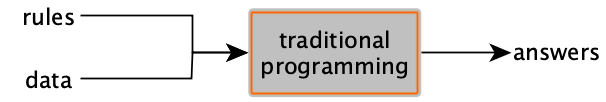
\includegraphics[width=100mm]{img/coli2020_diagrams_traditional_programming.png}
\end{center}

\btVFill
\footnotesize
Diagram borrowed from L. Moroney's Introduction to TensorFlow for Artificial Intelligence, Machine Learning, and Deep Learning
\end{frame}

\begin{frame}[fragile]
\frametitle{Introduction}
\framesubtitle{A simple method to \textit{salute} people}
\vspace{5mm}

\begin{block}{}
\begin{verbatim}
greeting_inputs = ("hey", "morning", "evening", "hi",
                "whatsup", "hello")
greeting_responses = ["hey", "hey hows you?", "*nods*",
                "hello, how you doing", "hello",
                "Welcome, I am good and you"]

def generate_greeting_response(input):
    for token in input.split():
        if token.lower() in greeting_inputs:
            return random.choice(greeting_responses)
\end{verbatim}
\end{block}

\onslide
\footnotesize
Derived from
\url{https://stackabuse.com/python-for-nlp-creating-a-rule-based-chatbot/}
\end{frame}


\begin{frame}
\centering
\alert{Unix for Poets}
\medskip

$\downarrow$
\medskip

\alert{Python for Poets}

\pause

\bigskip
\centering
\url{shorturl.at/iFMZ0}

\includegraphics[width=3cm]{img/01_coli2020_colab.png}

\end{frame}




\begin{frame}
\frametitle{References}
\bibliographystyle{humannat}
\bibliography{coli}
\end{frame}
\end{document}
